\documentclass[a4paper,11pt,uplatex]{jsbook}
%\usepackage{fancyhdr}
\setlength{\footskip}{16pt}
\usepackage{amsmath}
\usepackage[dvipdfmx]{graphicx}
\usepackage[dvipdfmx]{color}
%\usepackage{pagecolor}[white]
\usepackage{amsmath,amssymb}
%\usepackage[top=3cm, bottom=3cm, left=3cm, right=3cm]{geometry}
\usepackage{braket}
\usepackage{bm}
\numberwithin{equation}{section}
\usepackage{mathrsfs}
\usepackage{siunitx}
\usepackage{physics}
\usepackage[dvipdfmx]{graphicx}
\usepackage[compat=1.1.0]{tikz-feynhand}
\usepackage{caption}
\usepackage{subcaption}
%\usepackage{cleveref}
\usepackage{float}
\usepackage{multicol}
\setlength{\columnsep}{15mm}
%\usepackage[style=phys,articletitle=false,biblabel=brackets,chaptertitle=false,pageranges=false]{biblatex}
%\usepackage[style=phys]{biblatex}
\usepackage[dvipdfmx]{hyperref}
\usepackage{url}
\usepackage{pxjahyper}
\usepackage{bookmark}
%\usepackage[backref]{hyperref}
\setcounter{tocdepth}{3}
\setlength{\parindent}{2em}
\def\vector#1{\mbox{\boldmath $#1$}}
\def\slash#1{\not\!#1}
\def\slashb#1{\not\!\!#1}
\def\delsla{\not\!\partial}
%\usepackage[dvipdfmx]{xcolor}


\hypersetup{
 setpagesize=false,
 bookmarksnumbered=true,%
 bookmarksopen=true,%
 colorlinks=true,%
 linkcolor=black,
 citecolor=red,
 urlcolor=black,
}
%backreferenceのカスタマイズ. "Back to p.3"のように表示する.
%\renewcommand*{\backref}[1]{(p.#1へ戻る)}
%\newcommand{\backtoc}{\hyperlink{toc}{[目次へ]}}
\newcommand{\backtoc}{\texorpdfstring{\protect\hyperlink{toc}{\hspace{5pt} \scriptsize [目次へ]}}{}}
\newcommand{\mychapter}[1]{\chapter[#1]{#1\backtoc}}
\newcommand{\mysection}[1]{\section[#1]{#1\backtoc}}
\newcommand{\mysubsection}[1]{\subsection[#1]{#1\backtoc}}

\begin{document}
\chapter*{Appendix 回折計算}\label{chap:FFT}
\renewcommand{\theequation}{A.\arabic{equation}}
\setcounter{equation}{0}
\subsubsection{数値計算上の計算手法}

数値計算を実行する上では数値積分の手法では、伝搬後の$N$次元の配列が伝搬前の$N$次元配列全ての積分を用いて計算されるため計算量は$N^2$となる。
このような計算コストの高い計算を避けるために、高速フーリエ変換を用いた計算が一般に用いられている。
式(\ref{レイリーゾンマーフェルト近似})を再度$x,y,x_0,y_0$で書き直すと
\begin{eqnarray}
  U(x_0,y_0) \sim \frac{1}{2i\lambda zs}\int_S U(x,y) \exp( ik \sqrt{z^2 + (x-x_0)^2 + (y-y_0)^2}) dxdy
\end{eqnarray}
これはカーネル関数$f(x,y) = \sqrt{z^2 +x^2 + y^2}$であるような畳み込みの形で書ける。
\begin{eqnarray}
  U(x_0,y_0) \sim (U * f)(x,y)
\end{eqnarray}
畳み込みはフーリエ変換を用いることで
\begin{eqnarray}
  (U*f)(x,y) = \mathcal{F}^{-1}(\mathcal{F}(U) \times \mathcal{F}(f)) \label{convolution}
\end{eqnarray}
と表せる。ここで$\mathcal{F}$はフーリエ変換を表す。これは以下のように示すことができる。
\begin{eqnarray}
  (U*f)(x) = \int_{-\infty}^{\infty} U(t)f(x-t)dt
\end{eqnarray}
これをフーリエ変換したものは、
\begin{eqnarray}
  \mathcal{F}(U*f)(k) = \int_{-\infty}^{\infty} \int_{-\infty}^{\infty} U(t)f(x-t)dt \exp(-ikx)dx
\end{eqnarray}
積分の順序を交換して$x-t = y$とおくと、
\begin{eqnarray}
  \mathcal{F}(U*f)(k) &=& \int_{-\infty}^{\infty} U(t) \exp(-ikt)dt \int_{-\infty}^{\infty} f(y) \exp(-iky)dy\\
  &=& \mathcal{F}(U) \times \mathcal{F}(f)
\end{eqnarray}
したがって式(\ref{convolution})が示される。

フーリエ変換による計算では、空間領域($x,y$)の光波を周波数領域($k_x,k_y$)に変換する場合、空間領域の光波は計算に用いた空間領域を1周期とする周期的な光波として扱われている(図(a))。
そのため、そのまま逆変換を行うと隣り合う空間領域の光波が干渉してしまい、いわゆる円状畳み込みの結果を与える。これを防ぐために、計算空間の端を0で埋めた上で計算に用いる空間領域を拡大するゼロパディングを行うことで、(直線状)畳み込みの結果を得ることができる(図(b))。
\begin{figure}
  \centering
  \begin{subfigure}[h]{0.3\linewidth}
    \centering
    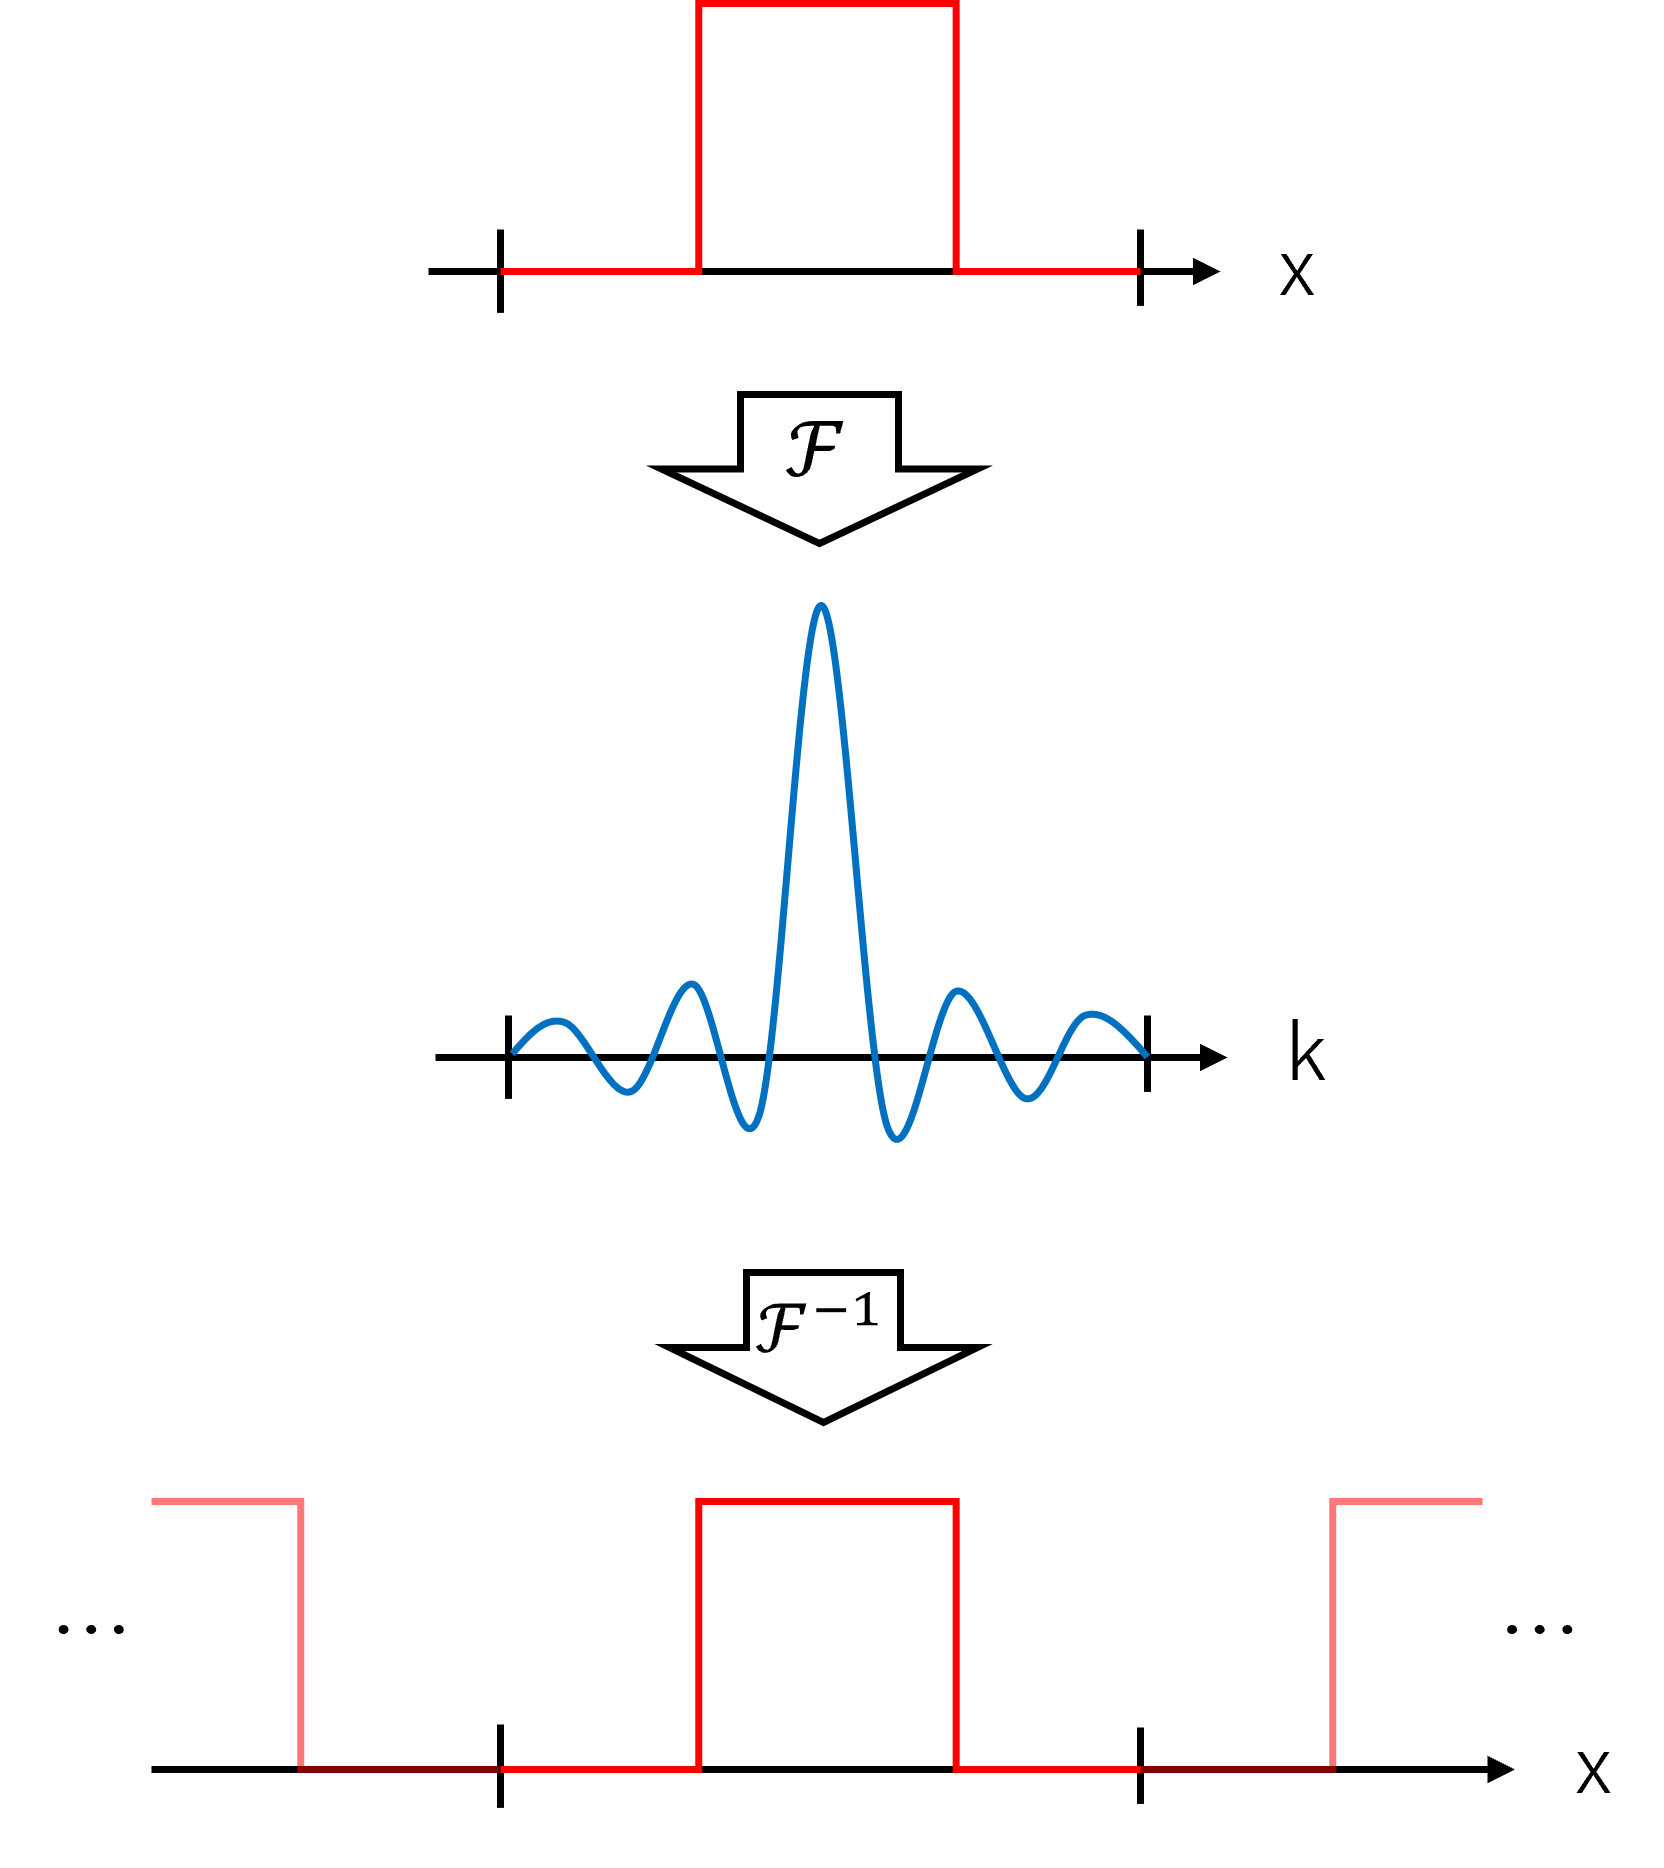
\includegraphics[width=\linewidth]{image/4-ft.png}
    \subcaption{円状畳み込み}
  \end{subfigure}
  \hfill
  \begin{subfigure}[h]{0.65\linewidth}
    \centering
    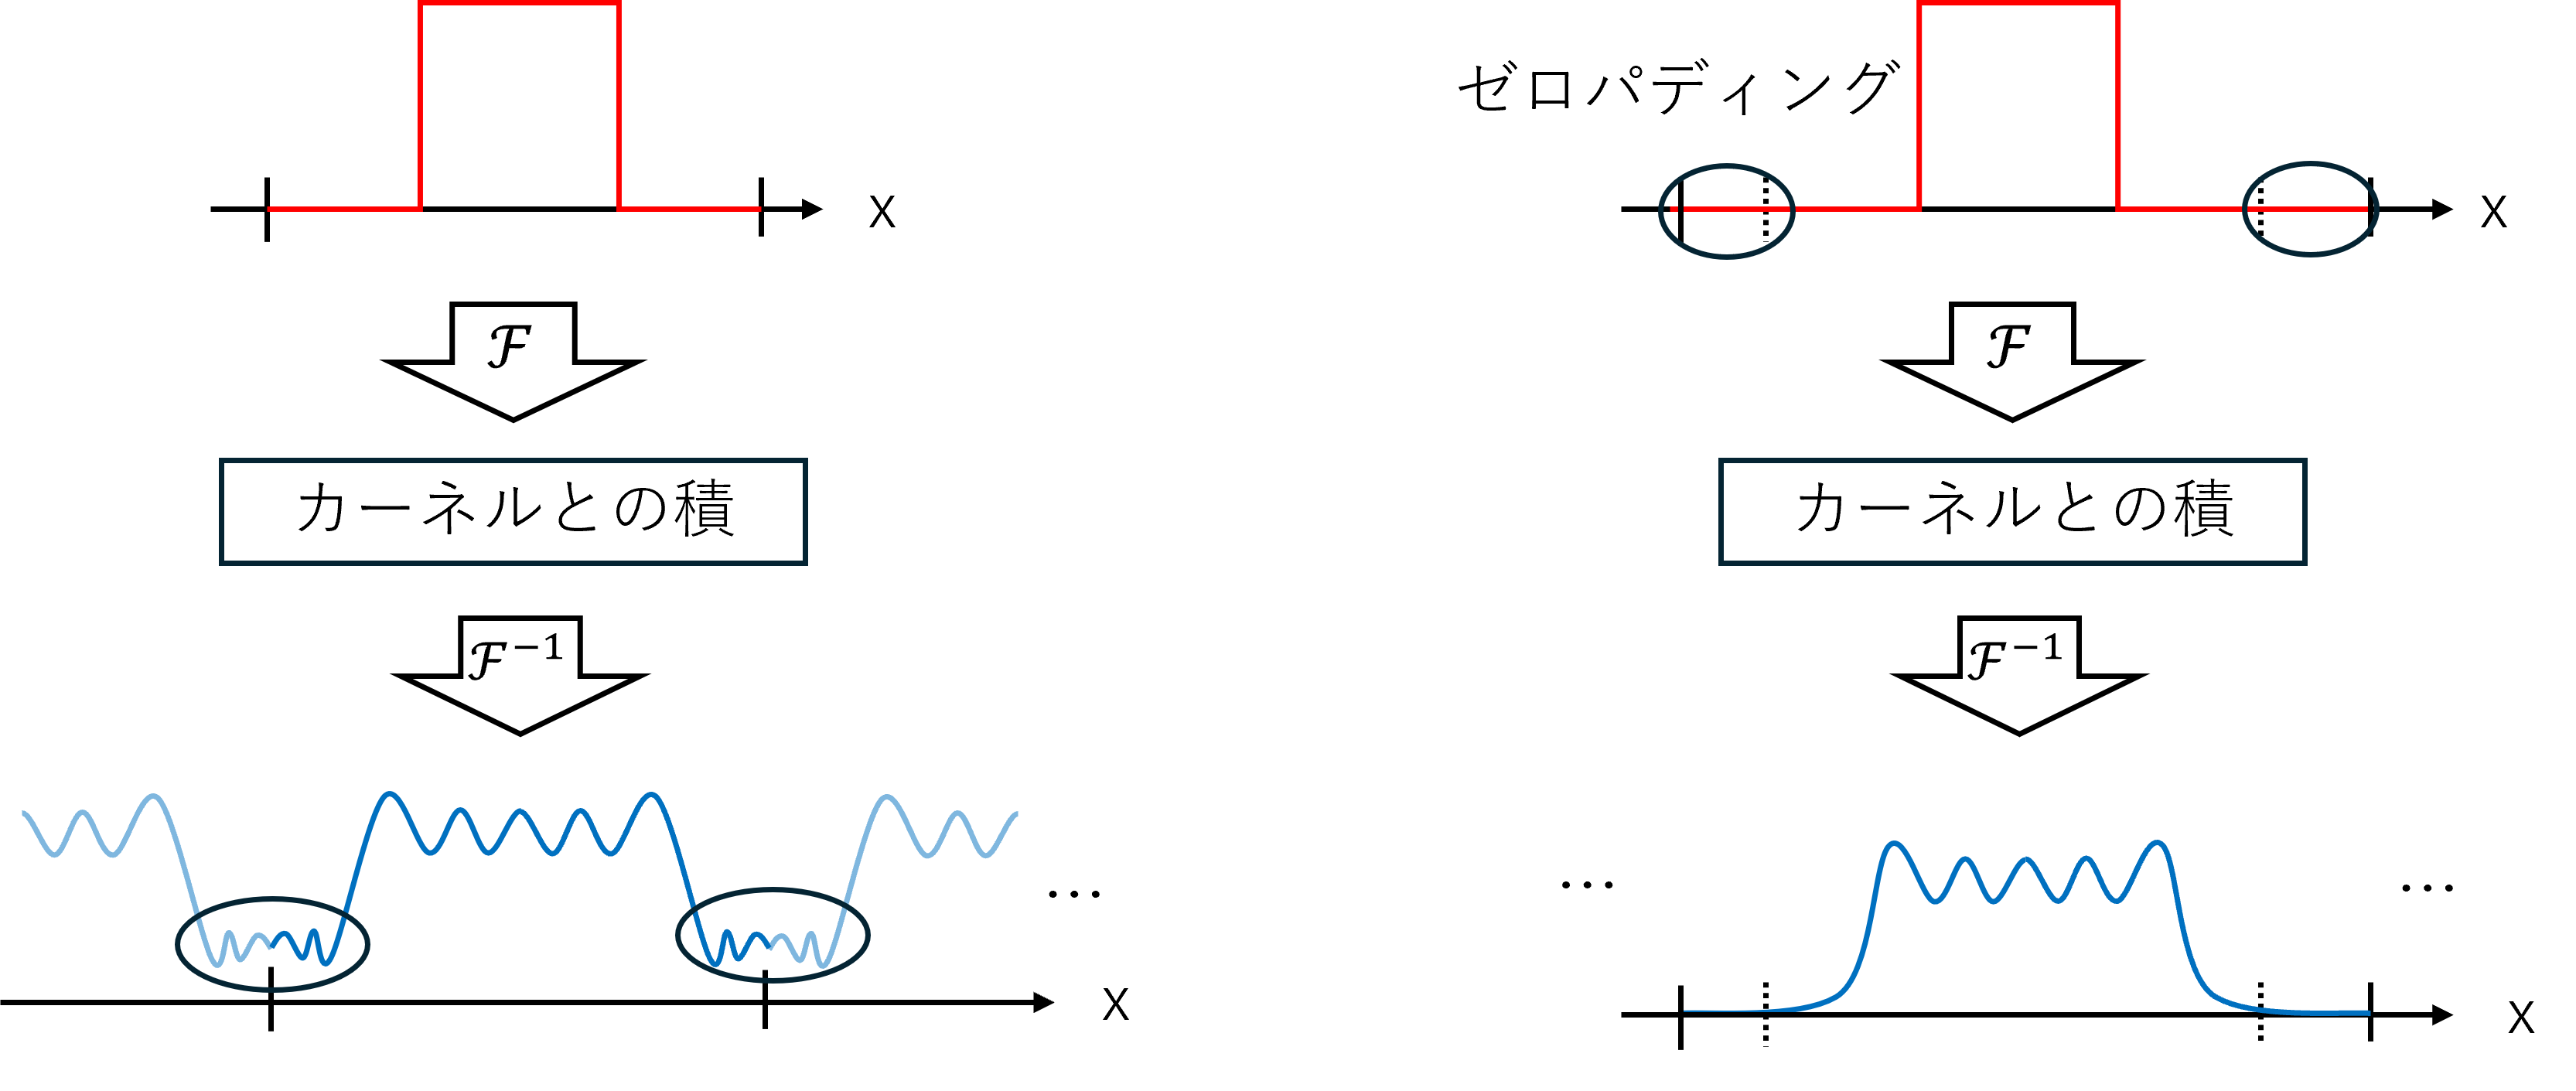
\includegraphics[width=\linewidth]{image/4-ft_zeropadding.png}
    \subcaption{ゼロパディング}
  \end{subfigure}
  \caption[フーリエ変換による畳み込みの数値計算]{フーリエ変換による畳み込みの数値計算。左図のように周波数領域では周期的な光波として扱われている。そのため、畳み込みを行うと隣り合う空間領域が干渉しあう。ゼロパディングを行うとこの干渉を抑制することができる。}
\end{figure}\label{ft}

\end{document}